\documentclass[conference]{IEEEtran}
\pagenumbering{roman}
\IEEEoverridecommandlockouts
% The preceding line is only needed to identify funding in the first footnote. If that is unneeded, please comment it out.
\usepackage{cite}
\usepackage{amsmath,amssymb,amsfonts}
\usepackage{algorithmic}
\usepackage{graphicx}
\usepackage{textcomp}
\usepackage{xcolor}
\def\BibTeX{{\rm B\kern-.05em{\sc i\kern-.025em b}\kern-.08em
    T\kern-.1667em\lower.7ex\hbox{E}\kern-.125emX}}
\begin{document}

\title{EECS4443 Project: SwipeNotes\\}

\author{
    \IEEEauthorblockN{Jerry Wu (217545898)}
    \IEEEauthorblockA{\textit{dept. of Electrical Engineering and Computer Science} \\
    \textit{York University}\\
    Toronto, Ontario, Canada \\
    jerrywu0@my.yorku.ca}
    \and
    \IEEEauthorblockN{Connor-Francis McGrath (216869133)}
    \IEEEauthorblockA{\textit{dept. of Electrical Engineering and Computer Science} \\
    \textit{York University}\\
    Toronto, Ontario, Canada \\
    connorm3@my.yorku.ca}
    \and
    \IEEEauthorblockN{Huy Vuong (217746801)}
    \IEEEauthorblockA{\textit{dept. of Electrical Engineering and Computer Science} \\
    \textit{York University}\\
    Toronto, Ontario, Canada \\
    huyvuong@my.yorku.ca}
    \and
    \IEEEauthorblockN{Marios Fokaefs (Supervising professor)}
    \IEEEauthorblockA{\textit{dept. of Electrical Engineering and Computer Science} \\
    \textit{York University}\\
    Toronto, Ontario, Canada \\
    fokaefs@yorku.ca}
}

\maketitle

\begin{abstract}
We built a note taking application called SwipeNotes on Android SDK 34. The application has the functionality of writing and saving notes using Realm DB. Our application provides two separate implementations for bolding and italicizing the text, one using conventional on screen buttons and context menus one would find in similar applications such as Apple notes, and the other was a gesture based mechanic using a SimpleOnGestureListener. In our trials we tasked our participants with typing and formatting text, measuring the completion time of the task. We found that the mean completion time for using traditional buttons was 23.12 seconds, whereas gesture functionality had a mean completion time of 21.85 seconds. Qualitative observations signified that participants enjoyed the gesture control, citing how natural and easy to learn they were. Additionally, CPU usage was also measured between the two options. For the button controls the CPU usage was 18.3\% while the mean CPU usage for gesture controls was 14.3\%.
\end{abstract}

\subsection*{Keywords}
\textit{mobile computing, android, gesture, gestural input, touchscreen, context menu, button, input methods, formatting, text formatting}


\section{Introduction}

\subsection{Why mobile computing is important}
Mobile computing is relevant and important because it is widespread around the world and it is convenient/easy to use. Nowadays we have access to powerful handheld devices that allow us to perform tasks that were previously only possible on enterprise grade computers a few decades ago such as word processing. \\

Although the areas where mobile computing is relevant seems to be endless, students in higher education can greatly take advantage of mobile devices and their many capabilities. Mobile devices assist students with gaining information and engaging with their learning both in and outside of the classroom [1]. The effect of mobile technologies is only predicted to grow as their computational power and opportunities for further learning engagement increases [1]. This is especially relevant for our current generation, where smartphone usage is rapidly increasing. Research shows that smartphone ownership across the globe increased by approximately 25\% from 2013 to 2016 [8]. Smartphones are especially common amongst university students, with around 86 to 94\% of higher education students owning smartphones in the US, UK, Australia, Saudi Arabia, and South Africa [8].

\subsection{Why note-taking apps are relevant}
A paramount aspect of the student experience is note taking. Although traditionally done on paper, the use of computer and mobile technology has become increasingly more popular throughout the years. Furthermore, for many university students, the time spent studying and learning independently is just as, if not more time consuming than the time spent in the classroom [1]. Therefore, it is important to provide students with note taking platforms and applications that are flexible and can be tailored to many different learning tasks and environments [1]. Note taking apps are relevant and important because they enable effective organization and productivity for the user. Note taking allows an end user to organize their thoughts in a brief and concise manner which in turn increases productivity.

\subsection{The importance of text formatting}
Good typing options allow students to take better notes. The amount of information that students record is proportional to the influence it has on their learning. This is not referring to the speed at which they are able to record said information, but rather how the student is able to pay attention while simultaneously recording said information. In summary, if students aren’t able to pay attention and take good notes at the same time, then statistically they will do poorly in their classes [8]. It is important for students to be able to create quality notes that can be easily understood for later reference [2], and simple verbatim transcription potentially inhibits good note taking, as instead of engaging with the learning material, students are simply copying what they read and hear [8]. This presents a need for note taking that allows students to engage with the educational content, and therefore increasing comprehension, while reducing cognitive stress in all other areas [6].


\subsection{The main idea of our app}
The problem we intend to solve with SwipeNotes is the user having to access menus intended for these important functions which distract from the main purpose of the application. One way that note takers aim to reduce cognitive stress, improve readability, improve organization, and increase productivity is through the use of text formatting. Formatting functions, such as: bolding, italicizing, changing font size and colour are important means for students to efficiently write notes that highlight important information, increasing the note quality, which in turn greatly increases learning comprehension [2].\\
\begin{figure}[ht]
    \centering
    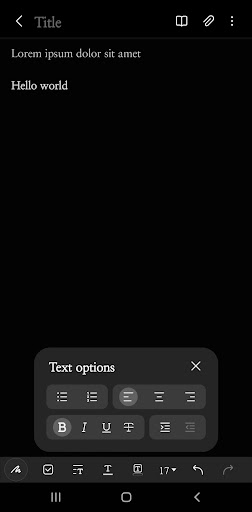
\includegraphics[scale=0.6]{images/textmenu.jpg}\\
    \caption{A context menu for changing text settings like bold, italic, etc. in Samsung Notes}
    \label{fig:enter-label}
\end{figure}

In terms of mobile text entry, there are several ways of reducing extraneous cognitive function that could be spent actively engaging with lectures. One such way is through the use of efficient on screen gestures as opposed to button input. Gestures can help alleviate issues that arise in most modern word processing applications. On a computer, a multitude of on screen buttons is usually not an issue since the user has more screen real estate to work with when using an application. However, on a mobile application, the screen real estate is a lot more restricted. Using gestures to access certain features rather than on screen buttons is especially important here since it minimizes the number of elements that are on the screen at any given time. For example, if a user were to make the text they write into a bold or italic, they would have to open a context menu with said options in the menu. This creates distraction from the main task at hand which is taking notes since there is a whole new menu on the screen glaring at the user. This will in turn reduce the overall productivity of the user.


\subsection{How is it different from conventional note apps?}

SwipeNotes differs from conventional note taking apps because it will replace important features such as bolding, font size changing, etc. that are usually locked behind on screen buttons to having them be accessed by gestures instead. The problem we intend to solve with this change is the user having to access menus intended for these important functions which distract from the main purpose of the application. Our design hopes to decrease the time between interactions, whether they be between keys or menus, which studies have previously shown increase WPM [5] and hopefully decrease time spent not engaging in lessons.

\begin{figure}[ht]
    \centering
    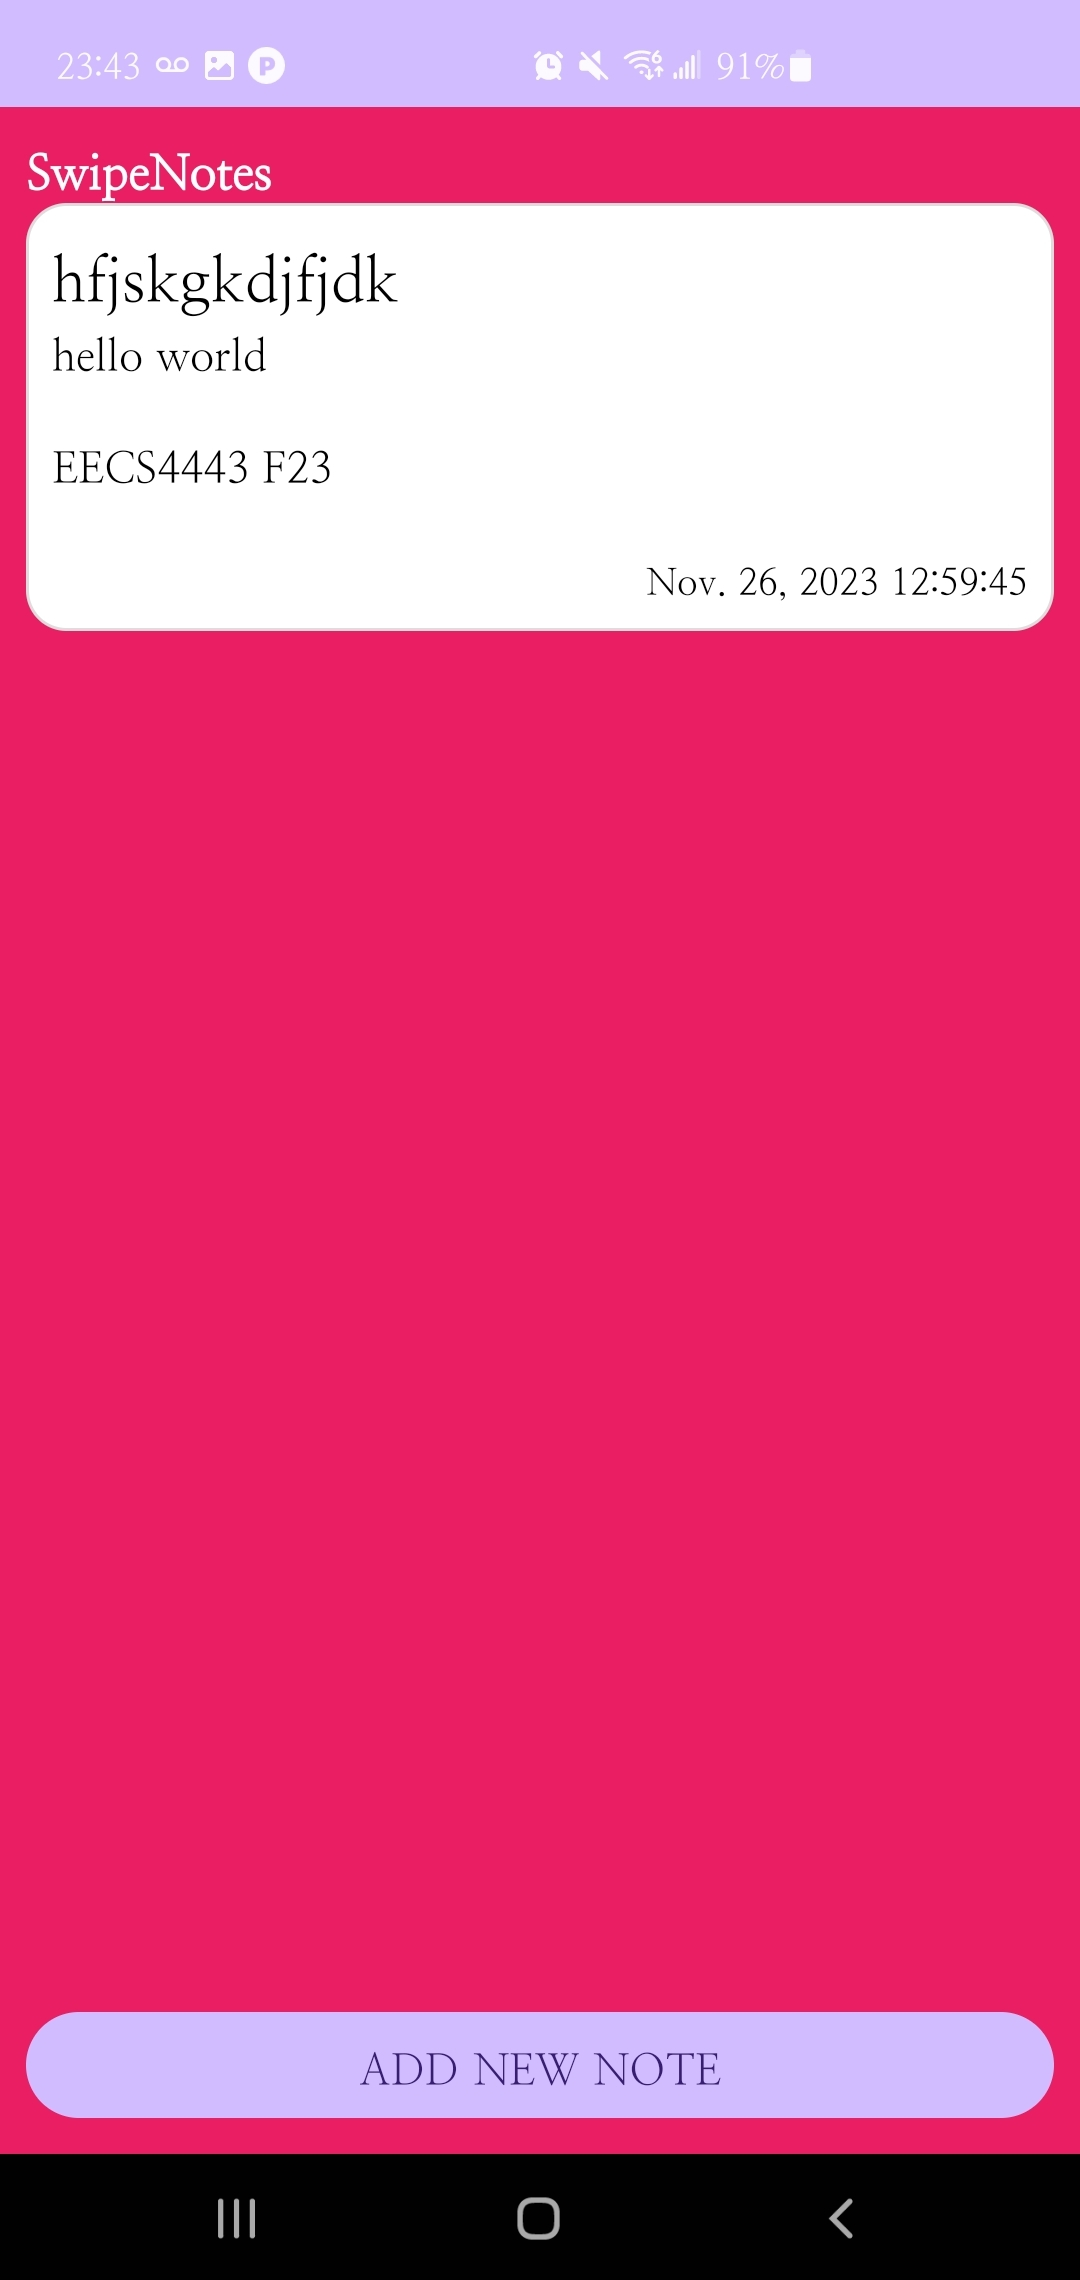
\includegraphics[scale=0.15]{images/notemenu.jpg}\\
    \caption{The note menu for SwipeNotes}
    \label{fig:enter-label}
\end{figure}


\subsection{How can gestures solve common barriers in note-taking?}

Gestures can help alleviate issues that arise in most modern word-processing applications. On a normal computer, a multitude of on-screen buttons is usually not an issue since the user has more screen real estate to work with when using an application. However, on a mobile application, the screen real estate is a lot more restricted. Using gestures to access certain features rather than on-screen buttons is especially important here since it minimizes the number of elements that are on the screen at any given time. For example, if a user were to make the text they write into bold or italic, they would have to open a context menu with said options in the menu. This creates distraction from the main task at hand which is taking notes since there is a whole new menu on the screen glaring at the user. This will in turn reduce the overall productivity of the user.


\begin{figure}[ht]
    \centering
    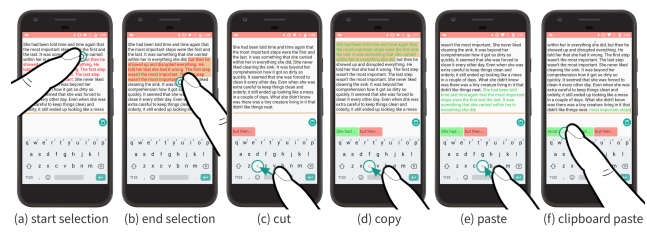
\includegraphics[scale=0.4]{images/gestures.png}\\
    \caption{An example of gestures replacing common functionalities with the application GeShort [4]}
    \label{fig:enter-label}
\end{figure}

\begin{figure}[ht]
    \centering
    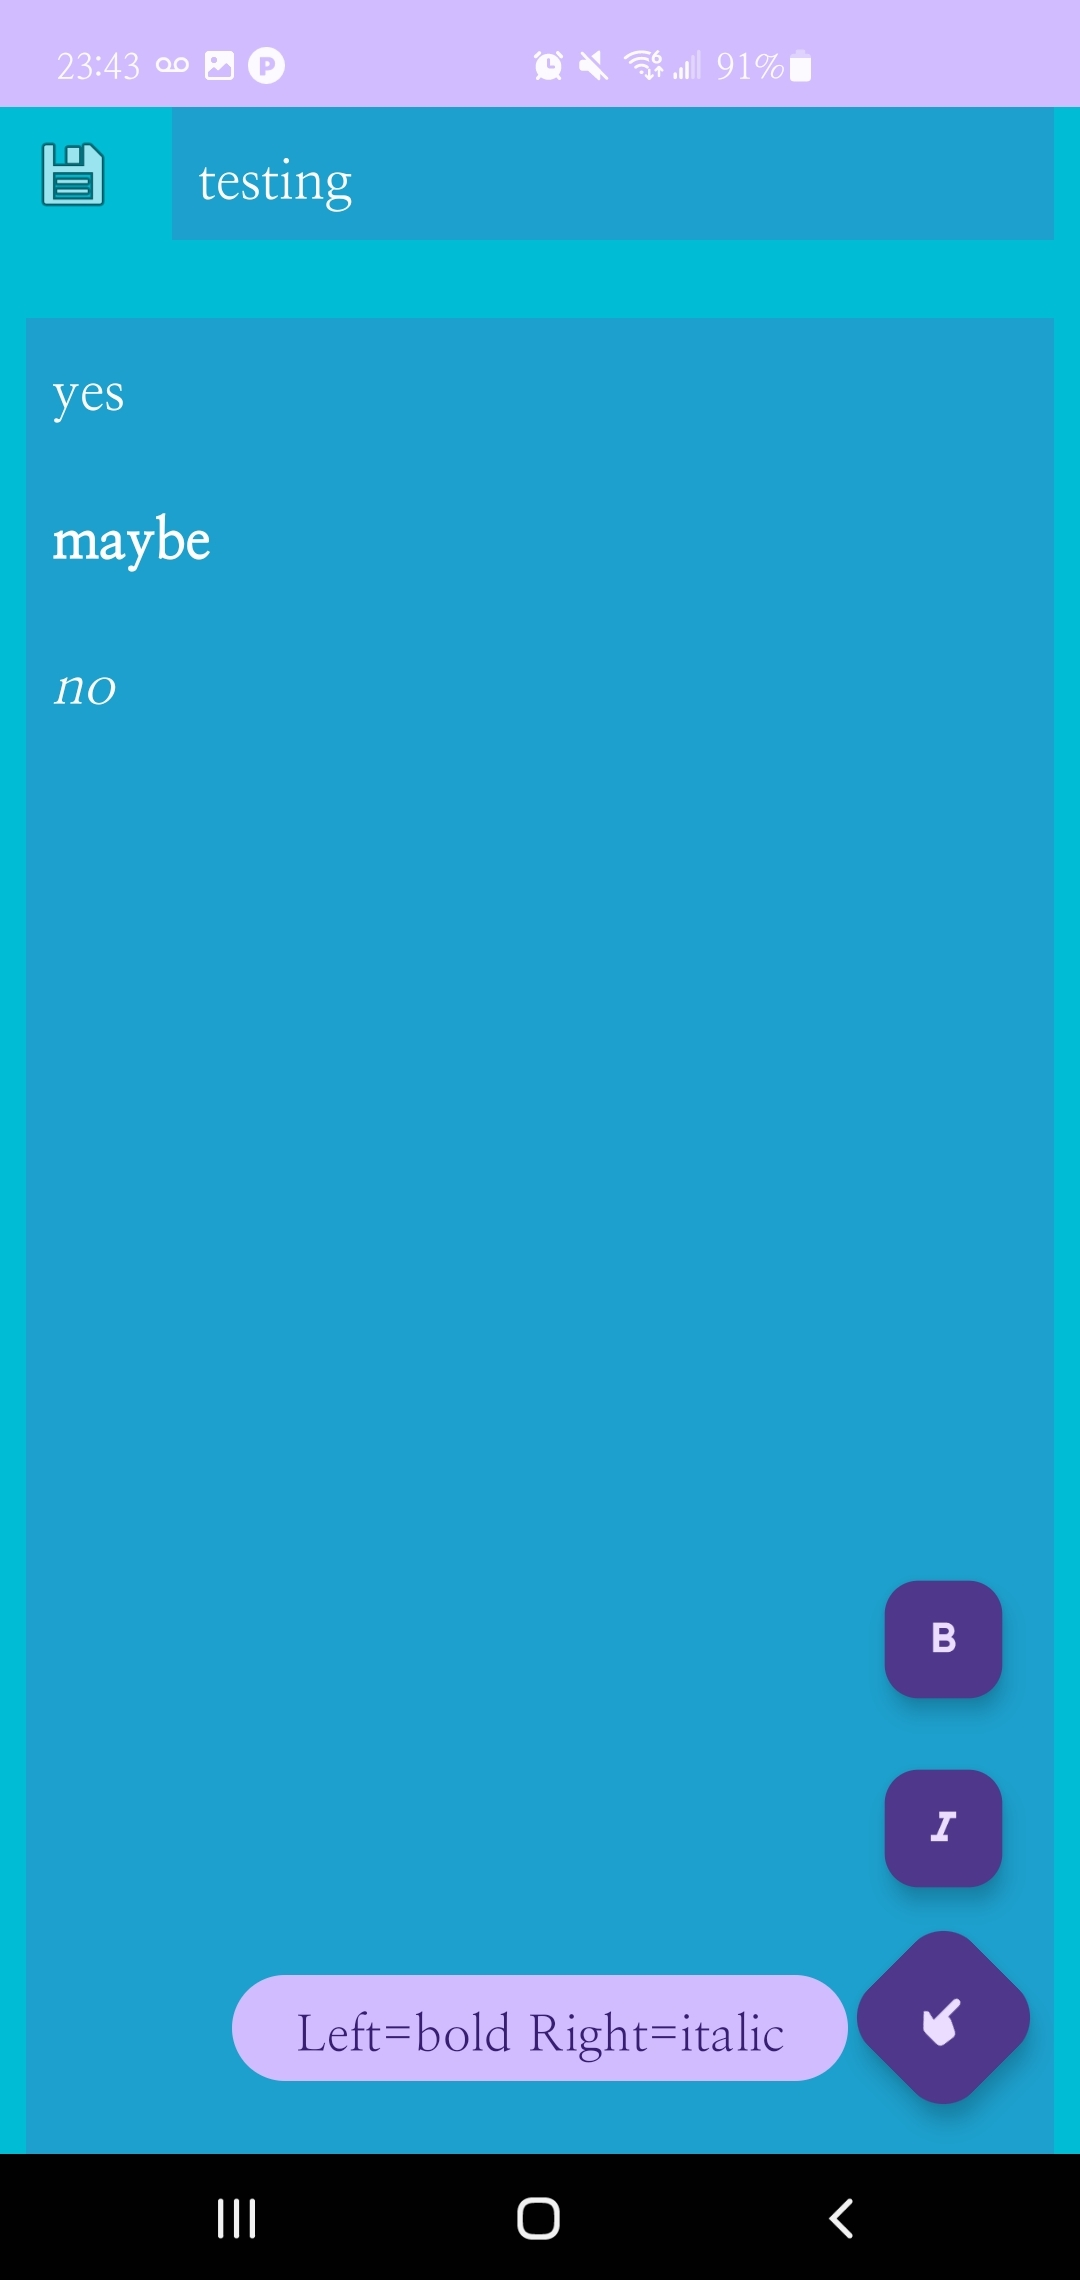
\includegraphics[scale=0.15]{images/editnote.jpg}\\
    \caption{The EditNoteActivity of SwipeNotes, featuring the context menu buttons on the bottom right for bold and italics along with the gesture bar at the bottom center for the same features.}
    \label{fig:enter-label}
\end{figure}

\subsection*{Related works}
\begin{figure}[ht]
    \centering
    \includegraphics[scale=0.65]{images/chart.png}\\
    \caption{Positives and negative qualitative feedback for gesture and keyboard based typing features found by experiments done by Reyal, Zhai, and Kristensson [7]}
    \label{fig:enter-label}
\end{figure}

The importance of note taking has been studied extensively. A study done with 93 middle school students highlighted the differences in note taking practices between higher achieving students, average achieving students, and students with learning disabilities [2]. The results of the study showed that predictably, the higher achieving students tended to take notes that captured the most important topics of the lectures more than their average achieving counterparts. The higher achieving students captured on average 52\% of the lecture points deemed critical, while the average achieving students captured 27\%. The study also suggested that writing meaningful notes has less to do with writing fluency and more to do with cognitive processing, and has the potential of making typing a much more cognitively challenging task [2]. The results of this study supports SwipeNotes’ goal of reducing the cognitive load of formatting to not only generate more seamless user experience, but also making the capturing and formatting of critical lecture points less taxing.
\\

SwipeNotes is not the first attempt to increase the effectiveness of mobile text entry. One example is GeShort, created at the University of California, a method for using gestures on the on-screen keyboard in order to edit and format text, inspired by keyboard hotkeys [4]. Their experiments with the product showed formatting and editing tasks to be approximately 11\% and 22\% faster than the Google keyboard [4]. Additionally, there were several qualitative observations from their participants that using gesture based text editing and formatting was less strenuous, faster, and easier to use than the default Google keyboard [4]. GeShort highlights how gesture based input can increase efficiency in text formatting and editing, as well as provide users with a better alternative than the formatting methods currently on the market.\\


Additionally, Unifone, a mobile device that utilizes squeeze gestures for common mobile tasks, including formatting. In the Unifone trials, the typical context menu for formatting text was compared to the gesture based actions of Unifone, where a squeeze gesture opened the context menu, and the formatting selection was made when the squeeze was released [3]. The results showed the Unifone completion times for the task were faster than the tapping alternative, with a mean completion time of 4.2 seconds for Unifone, and 5.62 seconds for the tapping input [3]. Another example of how completion time for the task of formatting can be significantly reduced by using gestures to replace the process of opening the context menu.\\


Lastly, Completion time is not the only factor to consider, but all aspects of the user experience while typing. A 2015 study [7] that compared the standard touch keyboard to a gesture keyboard in which the user slides their finger across the keyboard to spell words, presented many qualitative observations on the user’s experience with both styles of keyboard. Most importantly, one of the major critiques of the touch keyboard is the issue of accidentally tapping on keys or menu items the user did not intend to press [7]. SwipeNotes’ focus on gestures based text formatting aims to alleviate this issue by eliminating the need to press on screen buttons to open the context menu and select the right option.

\section{Method}
In order to ensure that our testing is thorough and relatable, we collected data from a sparse sample of users of different circumstances. Because this is not a large project, we collected data from a group of 10 individuals on York University's Keele campus, regardless of their gender, sex, or background. 8 out of 10 of them were EECS students, and the remaining 2 were in the department of Music in the AMPD faculty.

\subsection{Participants}
We selected 10 users, both male and female on the grounds of York University from the ages of 18-30 in the EECS department and the music department under AMPD. Each participant is categorized based on their specific needs and preferences regarding note-taking. This profiling will help us understand how different users interact with the application. The gesture-based note-taking feature of our application will be made available to users. During the time they are requested to use the app, they will type out exactly two (2) sentences containing 76 charaters (not including whitespace) and they will be timed for how fast they can type it out and format the first and second line with bold and italic respectively. This will be repeated for both formatting methods (buttons vs gestures). At the end, participants were asked how they liked using the gesture feature compared to conventional context menus to format notes, as well as how the app can be improved through further development. It will gather information on the convenience, effectiveness, and reduction of on-screen distraction and overall user satisfaction.

\subsection{Apparatus}

Due to time constraints, our participants tested the application in the following environment:
\begin{itemize}
    \item App was installed on a Samsung Galaxy S21 on Android SDK 34 with a 5.97x2.8 inch screen.
    \item The phone's CPU is a Snapdragon 888 5G with 8 GB of ram and 128 GB of internal storage.
    \item Each participant was timed using the stopwatch feature of the clock app on a Samsung Galaxy S10.
    \item The device was connected to a Razer Blade Stealth 14 with the Android Profiler running in the background to collect data about CPU usage.
    \item The laptop has a quad core 11th gen Intel Core i7 1165G7 @ 2.8GHz, 16GB of RAM, and 2TB of internal storage.
\end{itemize}   

\begin{figure}[ht]
    \centering
    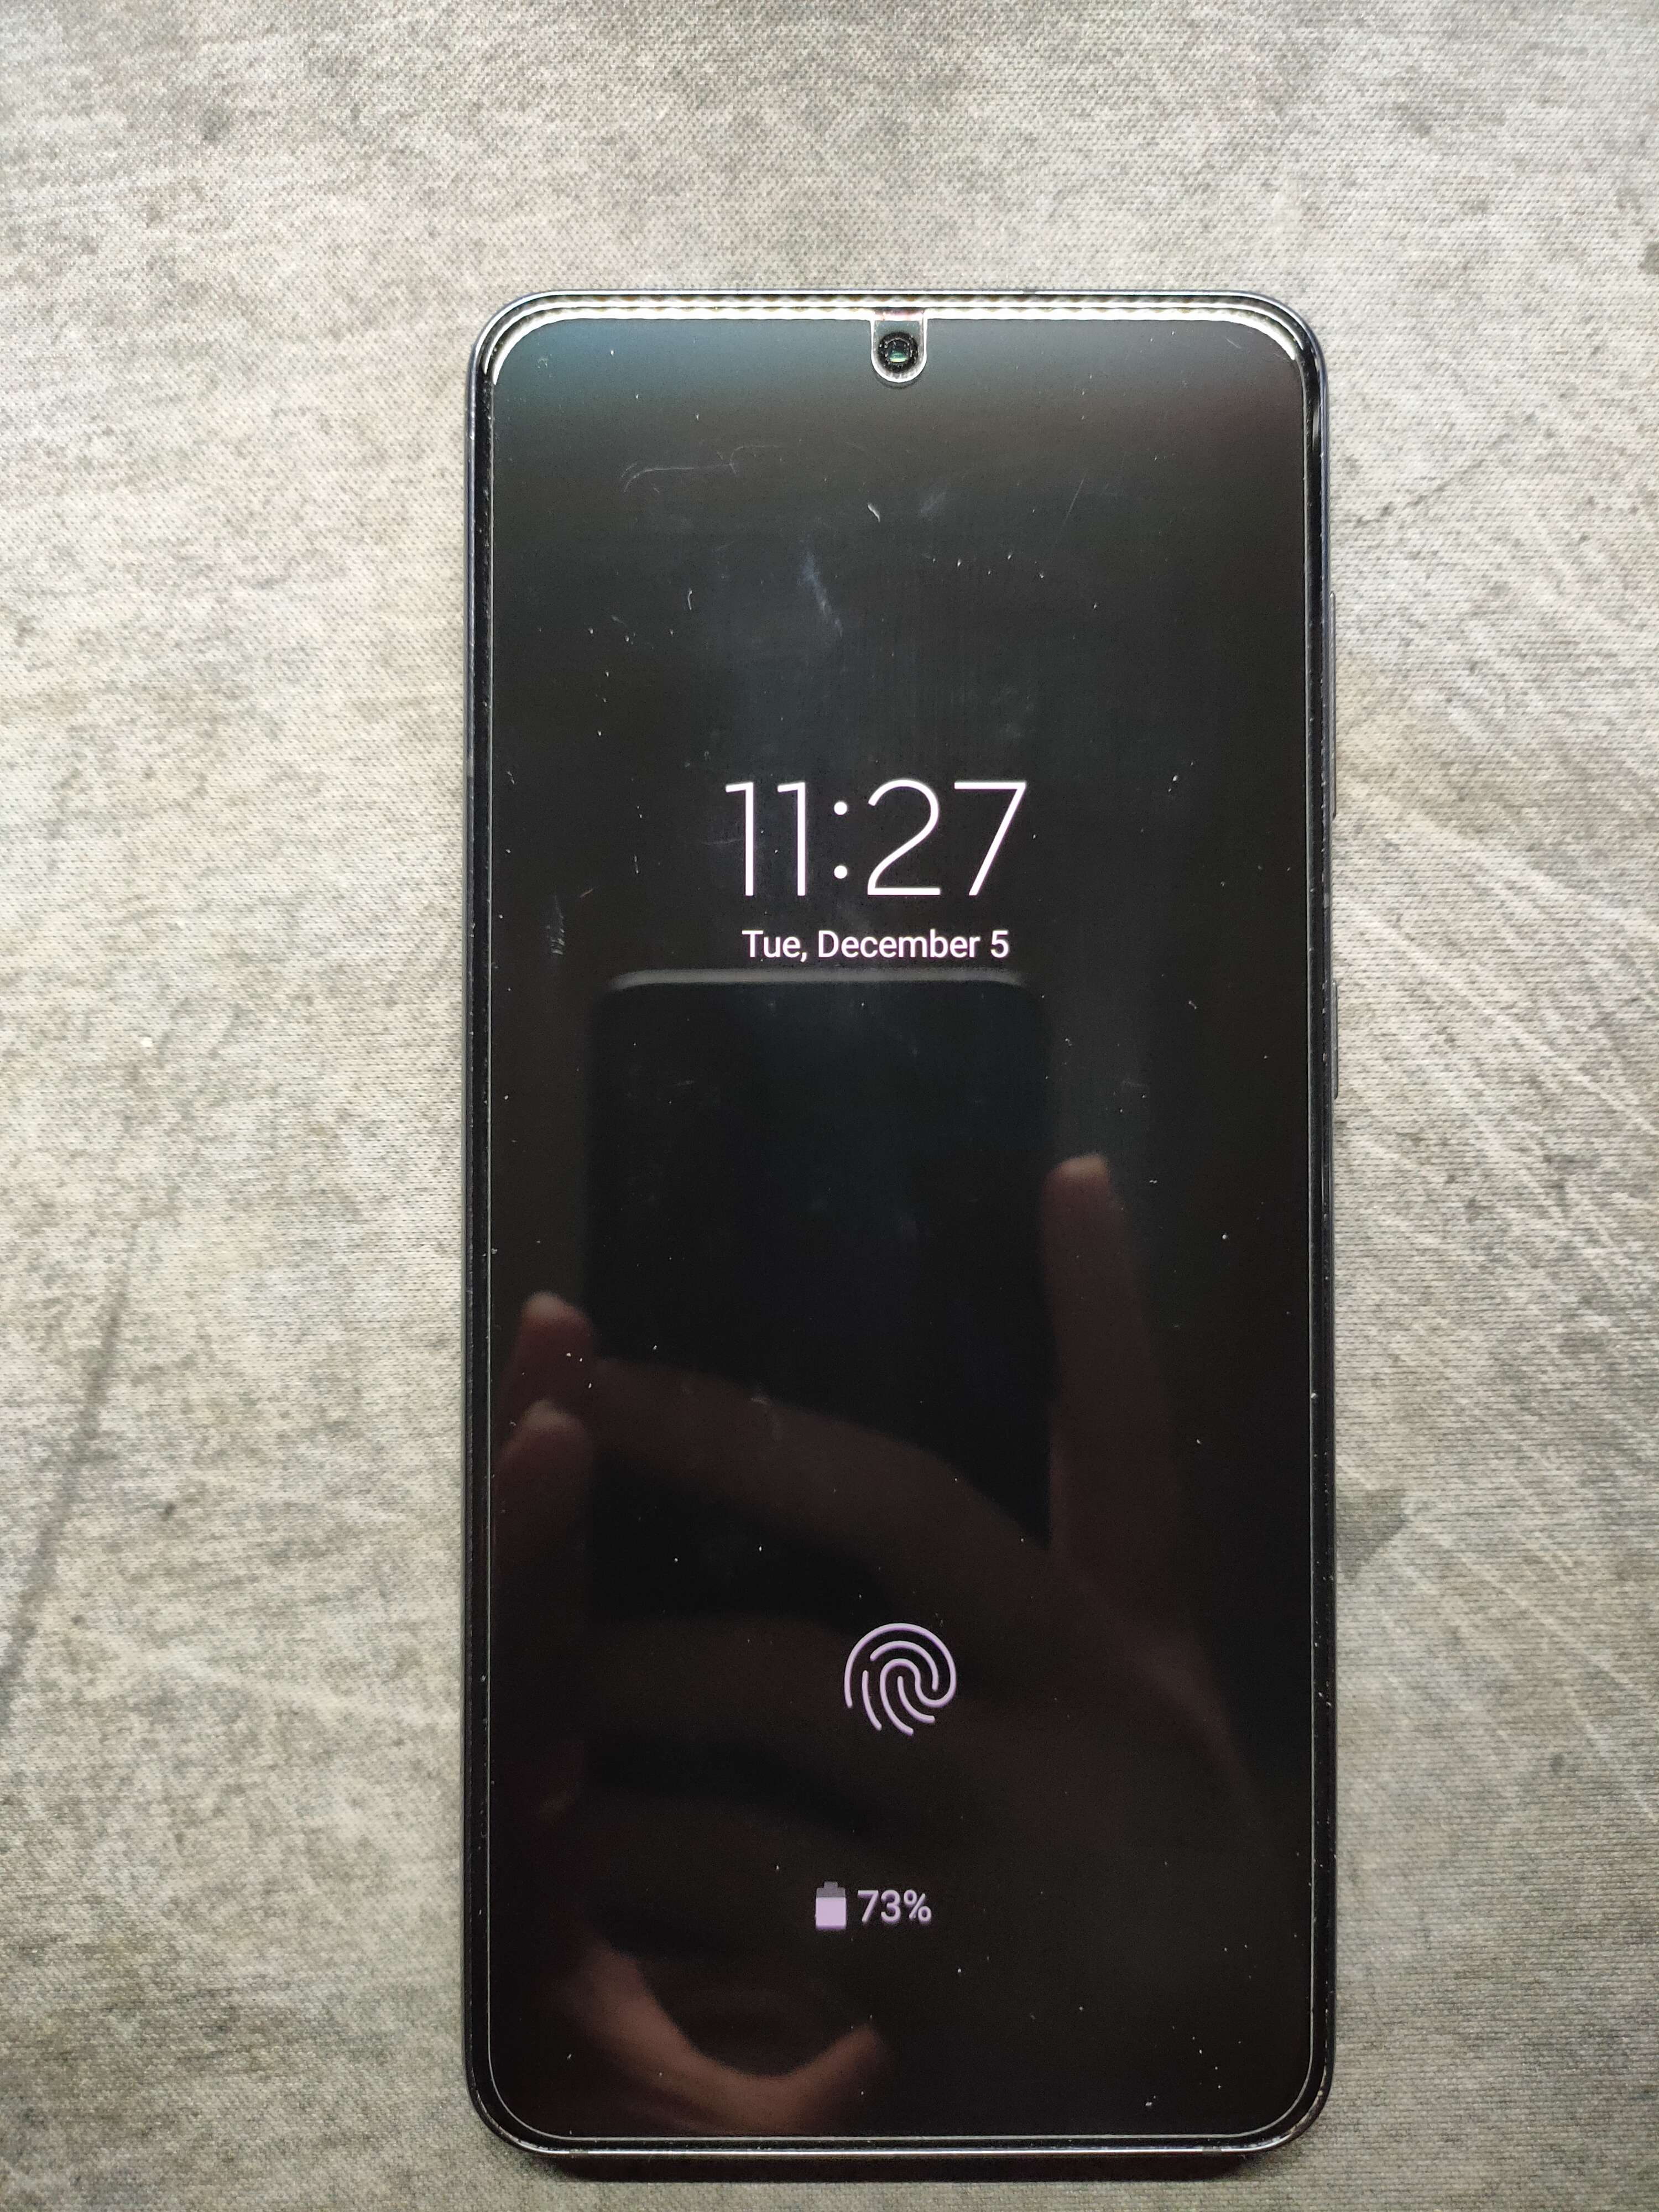
\includegraphics[scale=0.075]{images/s21front.jpg}\\
    \caption{The phone we used to test the application}
    \label{fig:enter-label}
\end{figure}

\begin{figure}[ht]
    \centering
    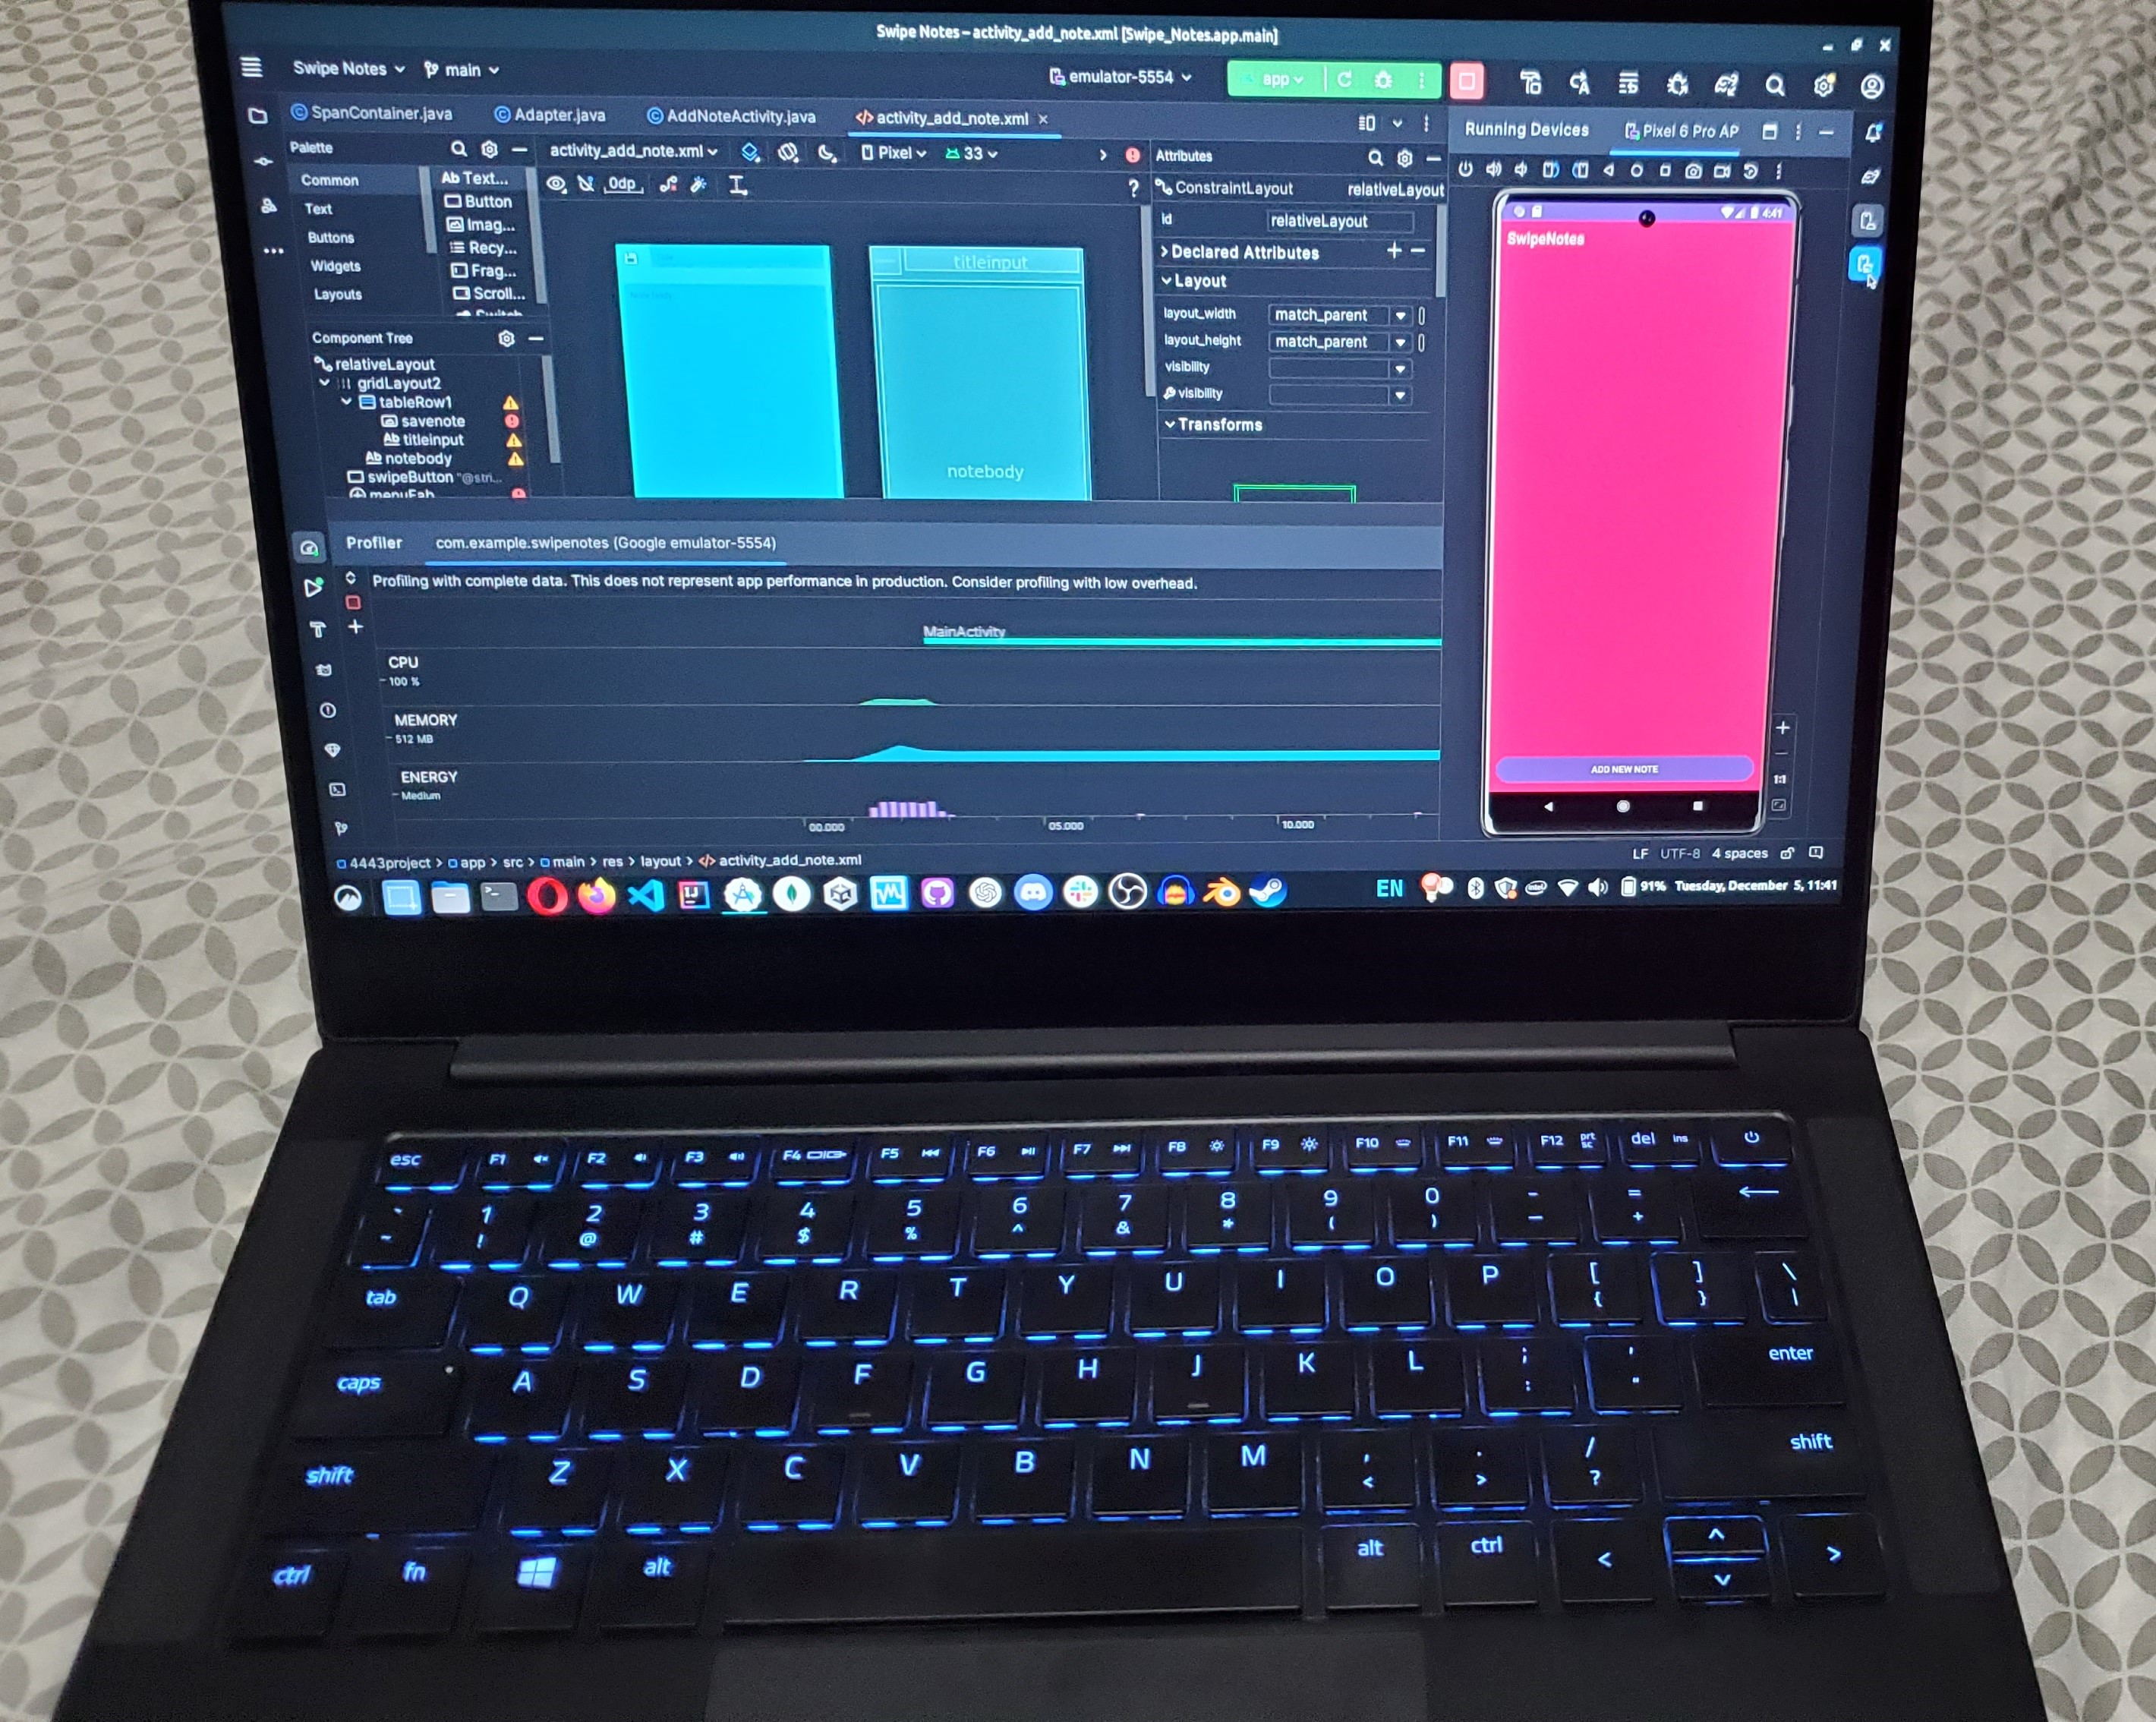
\includegraphics[scale=0.11]{images/laptop.jpg}\\
    \caption{The laptop we used to run the profiler alongside the application during testing with our participants}
    \label{fig:enter-label}
\end{figure}

\subsection{Procedure}

This section will detail the process of conducting our experiment with each participant.\\

\subsection*{What is the task?}
To preface, the task each participant will be performing is using both conventional buttons and a gesture bar to bold and italicize text typed out by the participant themselves. 

The sentences the participants typed out were the following:

\begin{itemize}
    \item [1.] \textit{"The only problem with troubleshooting is that sometimes trouble shoots back."}
    \item [2.] \textit{"During my exams, my calculator stopped working. I can't count on it anymore!"}
\end{itemize}

\subsection*{What is the goal of the task?}
The goal of performing this task is to measure the differences in the completion time of the formatting methods when performing it with buttons in a context menu as opposed to performing the task with our new method which is a gesture bar.

\subsection*{Starting and stopping of timing}
The stopwatch will be started when the user begins to type the sentences, and will stop once the user finishes italicizing the second line of the sentence. This applies to both formatting methods.

\subsection*{Were errors recorded?}
In terms of user error, there were generally typos that were made by users when typing each of the sentences. In terms of experimental errors, because we used a stopwatch to manually time participants for the experiment, there was most definitely error in the times, but we tried to be as accurate as possible by observing each participant closely and carefully for when they start and finish the task.

\subsection*{Were participants allowed to correct errors?}
Because making typos is a natural occurence in notetaking and typing as a whole, participants were allowed to correct their typos without the use of autocorrect. This time taken to correct said typos would be added to their final times for both trials as a result.

\subsection*{How were errors corrected?}
Errors were corrected in a variety of ways. Some participants would erase the word as a whole and re type it, while others would highlight the part they typed wrong and re type just that one part.

\subsection*{Were rest breaks allowed?}

Participants took a rest after finishing the first trial with bolding and italicizing with buttons and they let us know when they were ready to type the next sentence.

\subsection*{Instructions}

\begin{itemize}
    \item[1.] Participant enters the testing facility.
    \item[2.] Participant is given a device with the app installed on it.
    \item[3.] Participant will be given the task to type out a sentence that is 76 characters in length, bold the first line and italicize the second line with the conventional method (floating action buttons). Both sentences are written out by us, the testers in the editing panel so that the participant knew what they had to type out.
    \item[4.] Participant will then type out another sentence with the same number of characters (76 in total) and perform the same actions as in step 3, but this time using the gesture bar instead of the buttons.
    \item[5.] Steps 3 and 4 will be manually timed using a stopwatch, and the times it took to complete step 3 and 4 will be recorded and saved on a spreadsheet for later comparison and statistical analysis.
    \item[6.] Participant will be asked what they liked about using the application and what improvements can be made to it.
    \item[7.] Participant leaves the testing facility and will signal for the next participant to enter.
    \item[8.] Repeat all above steps until $n(participants)=0$.
\end{itemize}

\subsection{Design}
Each user typed out the \textbf{2} different sentences and will format the text with bold for the first line and italic for the second line. This leads to a within subject user study with a single independent variable with two levels for our experiment.



\begin{itemize}
    \item \textbf{Independent variables}: The IVs of this experiment are the two option change methods; conventional menu vs SwipeNotes gestures.
    \item \textbf{Dependent variables}: The DVs of this experiment are the task completion times with respect to both of the input methods.
\end{itemize}
To calculate the total number of trials, simply multiply number of participants (10) by number of input methods (2) and number of distinct trials per participant (1).
$n(trials)=10\times 1\times 2=20$

\subsection{User Hypothesis}

\begin{itemize}
    \item \textbf{Null hypothesis}: The difference in completion time of the formatting tasks will not be statistically significant between using gestures and using buttons for formatting.
    \item \textbf{Alternate hypothesis}: There will be a difference in completion time of the formatting tasks between using gestures and using buttons for formatting.
\end{itemize}

\subsection{Technical Hypothesis}

\begin{itemize}
    \item \textbf{Null hypothesis}: There will be no difference in CPU usage of the formatting tasks between using gestures and using buttons for formatting.
    \item \textbf{Alternate hypothesis}: The CPU usage of the formatting tasks will be different between using gestures and using buttons for formatting.
\end{itemize}

\section{Results \& Discussion}
\subsection{Results of the procedure}

\subsection*{User Hypothesis}

After asking 10 participants to use and test the app using the procedure, the result showed that, on average, people wrote faster when using gestures (21.85 seconds with 76 characters) than when using buttons (23.12 seconds with 76 characters). There was a 5.6\% decrease in completion time when using gestures over conventional buttons.
\begin{figure}[ht]
    \centering
    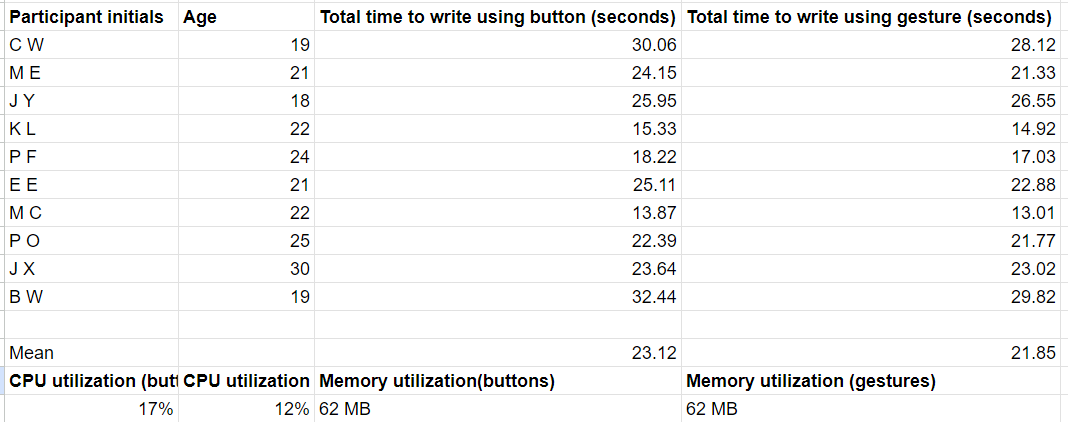
\includegraphics[scale=0.3]{images/table.png}\\
    \caption{The table containing all the raw data from the experiment including number of seconds each participant took for both methods.}
    \label{fig:enter-label}
\end{figure}

\begin{figure}[ht]
    \centering
    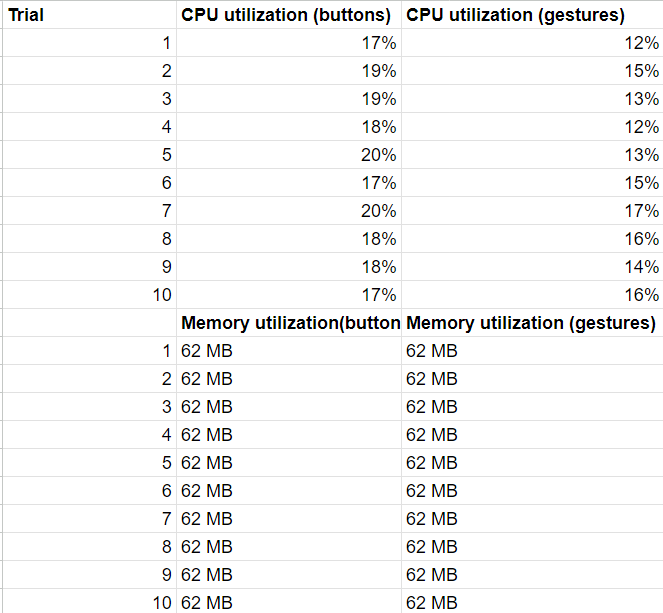
\includegraphics[scale=0.5]{images/cputable.png}\\
    \caption{The table containing all the raw data from the experiment for CPU/memory usage}
    \label{fig:enter-label}
\end{figure}

Each participant showed a decrease in the amount of time they took to complete the task, indicating that gestures are often more effective compared to buttons. After asking each participant which formatting method they liked using more, 9 out of 10 of them indicated that they liked the gesture bar more because of it's ease of use and fluidity. The one person who enjoyed using the context menu buttons more stated that they were simply just too adapted to using context menus to change their preferred way of formatting.\\

Given the fact that we had a categorical predictor variable, and a quantitative outcome variable with two groups we decided to run a t test. In this case a One Tailed Paired t Test:


Buttons\\
- Mean: 23.12 seconds\\
- Standard Deviation: 5.95\%

Gestures\\
- Mean: 21.85 seconds\\
- Standard Deviation: 5.55\%

t = 3.66

df = 9

p = 0.0052

$\alpha$ = 0.05

Because 0.0052 is less than 0.05, we can reject the null the hypothesis and determine that the difference in completion time between button and gesture controls is statistically significant.

\begin{figure}[ht]
    \centering
    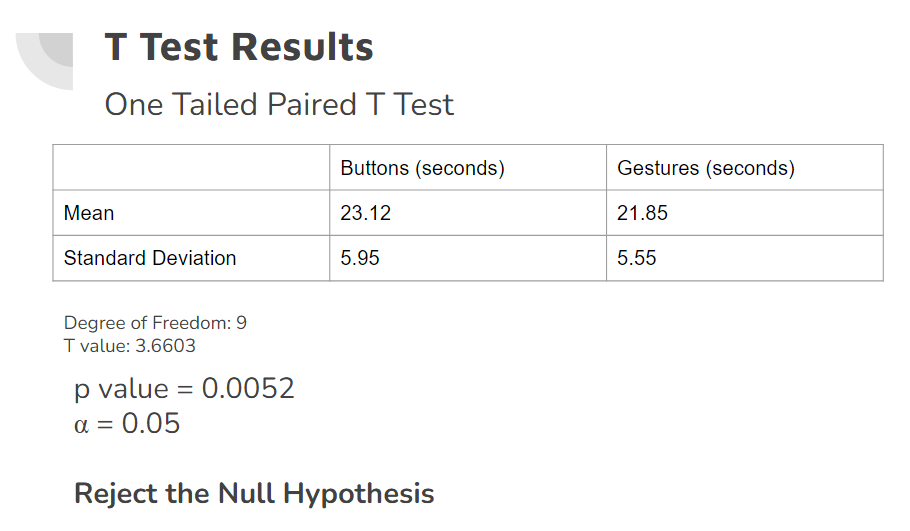
\includegraphics[scale=0.3]{images/results.png}\\
    \caption{Calculated results of the experiment based on a paired T test}
    \label{fig:enter-label}
\end{figure}

\subsection*{Technical Hypothesis}
\begin{figure}[ht]
    \centering
    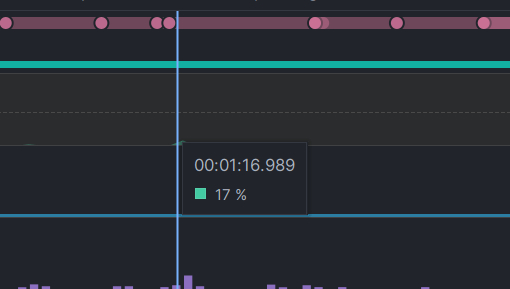
\includegraphics[scale=0.4]{profilerresults/cpuusage_btn.jpg}\\
    \caption{One of the trial results for CPU when formatting using buttons}
    \label{fig:enter-label}
\end{figure}

\begin{figure}[ht]
    \centering
    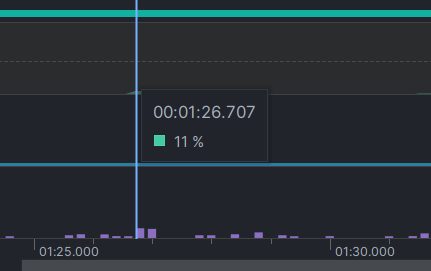
\includegraphics[scale=0.4]{profilerresults/cpuusage_gst.jpg}\\
    \caption{One of the trial results for CPU when formatting using gestures}
    \label{fig:enter-label}
\end{figure}

After 10 trials, the CPU usage was recorded using the Android Studio profiler. The mean CPU usage for the button controls was 18.3\%, while the mean CPU usage for the gesture controls was 14.3\%. Showing a 24.5\% difference in performance in favour of gestures when switching from button control to gesture control.

Similar to the user study, a one tailed paired t test was performed to see if the technical null hypothesis should be accepted or rejected.

Buttons\\
- Mean: 18.3\%\\
- Standard Deviation: 1.16\%

Gestures\\
- Mean: 14.3\%\\
- Standard Deviation: 1.77\%

t = -6.32

df = 9

p = 0.00006847

$\alpha$ = 0.05

Because 0.00006847 is less than 0.05, we can reject the null the hypothesis and determine that the difference in CPU usage between button and gesture controls is statistically significant.


\subsection*{Limitations}
We have talked about the ease of usage of gestures as a potential explanation for their superior performance. These results have significant interface design implications, favoring gestures as a more effective and user-friendly option. We acknowledge the study's limits and propose further investigation directions to guarantee that we keep learning about human-technology interactions.\\

One such limitation in this experiment is that participants were manually timed due to time constraints, as we didn't implement a feature to track number of seconds on board in the app itself. This makes the timing, our dependent variable, susceptible to human error.



\subsection{Discussion}
This section will detail some points of discussion relating to our app's performance based on the results we gathered from our experiment.

\begin{itemize}
    \item \subsection*{Performance (memory and CPU usage)}
    A very common point of discussion in mobile applications and apps in general is how they perform and how many system resources they use. Using the android profiler on our application, we followed the following procedure:

    \begin{itemize}
        \item Two different cases were used to gather the CPU and memory use data: the user interacting with the program using standard buttons and the user utilizing gesture controls. They were made in a controlled environment to guarantee that the measurements would result in accurate outcomes.
        
        \item The CPU usage during gesture control interaction is recorded at 14.3\%, while it increased to 18.3\% when users implemented standard buttons. This indicates that there is a 4\% decrease in CPU load resulting from the use of gesture controls. 
        
        \item The efficient handling of gesture inputs is responsible for the drop in CPU use, indicating that the implementation of gesture control is optimized and uses fewer system resources than button inputs. This enhancement shows that interacting with the application by gestures is not only a feasible option but also a more effective one compared to traditional buttons. 
    The amount of memory used for buttons and gestures in all circumstances stayed at 62 MB. This data shows that there aren't any differences in memory needs between the two interaction techniques for changing the text format of the input. The memory use stability indicated that it efficiently utilizes resources, guaranteeing a consistent user experience irrespective of the input method.
    \end{itemize}

    \item \subsection*{What caused differences in measurements across subjects?}
    The differences in measurements in our data suggest that some subjects have more experience with typing notes on mobile devices than other, as evident from the time they took to complete both tasks. Age had little to no correlation to the task completion time.

    \item \subsection*{Order effect?}
    Order effect may have had an impact on the speed at which participants were able to perform the 2nd part of the task with the gesture bar, as they were now familiar what the function of the gesture bar is given their prior experience with using the context menu buttons.

    \item \subsection*{Did one condition require more input actions?}

    The first task with formatting using buttons required more actions from the user than the gestures, as the user had to open the context menu by clicking the context menu button, then proceed to click on one of the formatting options. Conversely, the user simply had to swipe a finger along the gesture bar without opening any context menus to format using the 2nd method.

    \item \subsection*{Confusion among participants?}

    Fortunately this phenomenon was not exhibited throughout any of the 10 trials, as the task was simple enough to which a short explanation as to which lines to format with which formatting type (bold or italic) was sufficient enough. It should also be noted that we the testers wrote out the sentences on the phone so that the participant could give it a read before we timed them for the tasks. Incidentally, this is because of how intuitive it was to learn the method to begin with.

    \item \subsection*{Fatigue and exhaustion?}

    Because we live in an age where people use their phones to message people multiple times a day, none of the participants experienced any fatigue or exhaustion. It could also be that the task was relatively short, as the application isn't a large scale one.
    
\end{itemize}

\section{Conclusion}
\subsection{Findings}
SwipeNotes is an note taking app that allows for bold and italic text formatting using buttons, similar to other note taking apps on the market, with our own addition of gesture based swipe controls in order to format text as well.

Our user study contained a single independent variable with two levels, those being the two methods of formatting text.

In our study, we found that the use of gestures had a general decrease in the amount of time it took participants to format the text as compared to the traditional method of using buttons and context menus. Gesture controls reported a mean completion time of 21.85 seconds, whereas buttons achieved a mean completion time of 23.12 seconds.

Although there were users who admitted familiarity and comfort with traditional formatting methods, the user population as a whole expressed that SwipeNotes' gesture based controls were easy to learn and felt natural.

When looking at the impact on CPU usage, the mean CPU usage over 10 trials of button controls was 18.3\% while the mean usage for gesture controls was 14.3\%.

Our findings were in line with GeShort, a similar gesture based text formatting method mentioned in our related works section in the introduction. The University of California found that their solution provided faster formatting and editing features compared to the standard Google keyboard [4]. Our participants also echoed similar qualitative sentiments about how gesture based text formatting was easier and more natural to use [4].

Within our experiment we explore gesture based controls for text formatting. In further studies and trials of gesture based controls, additional features, such as paragraph formatting in the form of adding bullet points, indents, or horizontal lines using SwipeNotes gesture controls. The effects of our study and many others have shown the benefit of gesture controls, so their use in greater text formatting functionality should be explored in greater detail.





\begin{thebibliography}{00}
\bibitem{b1} Schepman, A., Rodway, P., Beattie, C., and Lambert, J., “An observational study of undergraduate students’ adoption of (mobile) note-taking software,” Computers in Human Behavior, vol. 28, no. 2, pp. 308–317, Mar. 2012, doi: https://doi.org/10.1016/j.chb.2011.09.014.
\bibitem{b2} Boyle, J. R., Forchelli G. A., “Differences in the note-taking skills of students with high achievement, average achievement, and learning disabilities,” Learning and Individual Differences, vol. 35, pp. 9–14, Oct. 2014, doi: https://doi.org/10.1016/j.lindif.2014.06.002.
\bibitem{b3} Holman, D., Hollatz, A., Banerjee, A., and Vertegaal, R., “Unifone: designing for auxiliary finger input in one-handed mobile interactions,” Proceedings of the 7th International Conference on Tangible, Embedded and Embodied Interaction, pp. 177–184, Feb. 2013. doi:10.1145/2460625.2460653 
\bibitem{b4} Rakhmetulla, G., Ren, Y., and Arif, A. S., “GeShort: One-Handed Mobile Text Editing and Formatting with Gestural Shortcuts and a Floating Clipboard,” Proceedings of the ACM on human-computer interaction, vol. 7, no. MHCI, pp. 1–23, Sep. 2023, doi: https://doi.org/10.1145/3604259.
\bibitem{b5} Palin, K., Feit, A. M., Kim, S., Kristensson, P. O., and Oulasvirta, A., “How do People Type on Mobile Devices?,” Proceedings of the 21st International Conference on Human-Computer Interaction with Mobile Devices and Services - MobileHCI ’19, 2019, doi: https://doi.org/10.1145/3338286.3340120.
\bibitem{b6} Mueller, P. A., and Oppenheimer, D. M., “Technology and note-taking in the classroom, boardroom, hospital room, and courtroom,” Trends in Neuroscience and Education, vol. 5, no. 3, pp. 139–145, Sep. 2016, doi: https://doi.org/10.1016/j.tine.2016.06.002.
‌
\bibitem{b7} Reyal, S., Zhai, S., and Kristensson, P. O., “Performance and User Experience of Touchscreen and Gesture Keyboards in a Lab Setting and in the Wild,” Human Factors in Computing Systems, Apr. 2015, doi: https://doi.org/10.1145/2702123.2702597.
\bibitem{b8} van Wyk, M., and van Ryneveld, L., “Affordances of mobile devices and note-taking apps to support cognitively demanding note-taking,” Education and Information Technologies, vol. 23, no. 4, pp. 1639–1653, Jan. 2018, doi: https://doi.org/10.1007/s10639-017-9684-0.
‌

\end{thebibliography}



\end{document}https://www.overleaf.com/project/655e4eec7a17ea2a3d9ab004